\documentclass[preprint,12pt]{elsarticle}

\usepackage[T1]{fontenc}
\usepackage[utf8]{inputenc}
\usepackage{amsmath}
\usepackage{amssymb}
\usepackage{bm}
\usepackage{booktabs}
\usepackage{graphicx}
\usepackage{mathtools}
\usepackage{microtype}
\usepackage{url}

\setlength{\emergencystretch}{2em}

\journal{ICMSEP 2026}

\begin{document}

\begin{frontmatter}

\title{Supplementary Material for ``Compatibility of Spectral and Operator
Reductions of Periodic Hamiltonians: Controlled One- and Two-Dimensional
Benchmarks''}

\author[dlsu]{Eugene Joseph M. Ragasa\corref{cor1}}
\ead{eugene.ragasa@dlsu.edu.ph}
\cortext[cor1]{Corresponding author.}

\address[dlsu]{Department of Physics, De La Salle University,
Manila, Philippines}

\end{frontmatter}

\section*{Appendix S1. Gauge-Orbit Diagnostic Decomposition}
\label{supp:orbit-diagnostic}
\renewcommand{\theequation}{S1.\arabic{equation}}
\setcounter{equation}{0}

\subsection*{S1.1 Purpose and scope}

This appendix defines the invariant and frame-dependent parts of the operator
comparison used in the main paper. The decomposition applies to the diagnostic,
not to the Hamiltonian as a physical operator. It is defined relative to a
frozen comparison contract; changing the retained space, admissible alignment
family, weights, normalization, or finite translation domain changes the
diagnostic.

The construction is analogous in purpose to the separation of the Wannier
spread into gauge-invariant and gauge-dependent contributions
\cite{marzari1997,marzari2012,panati2013}. It is not the Wannier spread
functional and does not inherit that functional's physical or variational
interpretation.

\subsection*{S1.2 Comparison contract}

Let $V_{\mathrm{ref}}$ and $V_{\mathrm{red}}$ be retained finite-dimensional
state spaces of equal rank $r$. The operator channel requires a nonempty,
declared family
\[
 \mathcal U\subseteq
 \left\{\bm C:V_{\mathrm{red}}\rightarrow V_{\mathrm{ref}}
 \mid \bm C^\dagger\bm C=\bm C\bm C^\dagger=\bm I_r\right\}
\]
of admissible unitary identification maps. Restrictions imposed by continuity,
reciprocal-boundary sewing, symmetry, orbital semantics, or locality belong to
the definition of $\mathcal U$ rather than to a later interpretation of the
residual.

For a finite translation domain $\mathcal S_H$, nonnegative weights
$\omega_{\bm R}$, and a positive frozen normalization
\[
 Z_{\mathrm{ref}}=
 \sum_{\bm R\in\mathcal S_H}\omega_{\bm R}
 \left\|\bm H_{\mathrm{ref}}(\bm R)\right\|_{\mathrm F}^2,
\]
the aligned operator loss is
\begin{equation}
 \mathcal L_H(\bm C,\bm\theta)=
 \frac{1}{Z_{\mathrm{ref}}}
 \sum_{\bm R\in\mathcal S_H}\omega_{\bm R}
 \left\|
 \bm H_{\mathrm{ref}}(\bm R)
 -\bm C\bm H_{\mathrm{red}}(\bm R;\bm\theta)\bm C^\dagger
 \right\|_{\mathrm F}^2.
 \label{eq:supp-aligned-loss}
\end{equation}
A zero or unspecified normalization does not define this diagnostic. A
different-rank comparison likewise requires a separately declared projection
or embedding; its information loss cannot be absorbed into
Eq.~\eqref{eq:supp-aligned-loss}.

\subsection*{S1.3 Orbit loss and frame excess}

\paragraph{Attainment under a compact contract.}
For fixed $\bm\theta$, the finite-sum loss in
Eq.~\eqref{eq:supp-aligned-loss} is a continuous real-valued function of
$\bm C$. If $\mathcal U$ is nonempty and compact, the extreme-value theorem
therefore supplies $\bm C_\star\in\mathcal U$ such that
\begin{equation*}
 \inf_{\bm C\in\mathcal U}\mathcal L_H(\bm C,\bm\theta)
 =\min_{\bm C\in\mathcal U}\mathcal L_H(\bm C,\bm\theta)
 =\mathcal L_H(\bm C_\star,\bm\theta).
\end{equation*}
In the finite-rank contract used here, $U(r)$ is compact, so it is sufficient
for the admissible family to be a nonempty closed subset of $U(r)$. Sewing,
symmetry, site, and orbital restrictions imply this conclusion only when their
frozen constraint maps define a closed set; the names of those restrictions do
not by themselves prove compactness. For a merely nonempty noncompact family,
the nonnegative loss still has a well-defined infimum, but a minimizing
alignment need not exist.

For nonempty $\mathcal U$, define the contract-invariant orbit loss
\begin{equation}
 \mathcal L_{H,\mathrm{orb}}(\bm\theta)
 =\inf_{\bm C\in\mathcal U}\mathcal L_H(\bm C,\bm\theta).
 \label{eq:supp-orbit-loss}
\end{equation}
For a particular declared alignment $\bm C_0\in\mathcal U$, define the
frame-dependent excess
\begin{equation}
 \mathcal L_{H,\mathrm{frame}}(\bm C_0,\bm\theta)
 =\mathcal L_H(\bm C_0,\bm\theta)
 -\mathcal L_{H,\mathrm{orb}}(\bm\theta).
 \label{eq:supp-frame-excess}
\end{equation}
For every $\bm C_0\in\mathcal U$, the defining greatest-lower-bound
property gives
$\mathcal L_{H,\mathrm{orb}}(\bm\theta)\leq
\mathcal L_H(\bm C_0,\bm\theta)$. Subtraction therefore proves
\begin{equation}
 \mathcal L_H(\bm C_0,\bm\theta)
 =\mathcal L_{H,\mathrm{orb}}(\bm\theta)
 +\mathcal L_{H,\mathrm{frame}}(\bm C_0,\bm\theta),
 \qquad
 \mathcal L_{H,\mathrm{frame}}\geq 0.
 \label{eq:supp-loss-decomposition}
\end{equation}
This is an exact scalar decomposition of the diagnostic. It is not an
orthogonal decomposition of the residual matrix.

The orbit term is the greatest lower bound of the operator discrepancy over the
frozen admissible family. The frame term measures the excess associated with
the selected admissible representative. Both statements are relative to
$\mathcal U$: enlarging the family can decrease the orbit loss, while adding
physical restrictions can increase it.

\subsection*{S1.4 Frame invariance}

Consider independent frame changes $\bm A$ on $V_{\mathrm{ref}}$ and $\bm B$
on $V_{\mathrm{red}}$. They transform the represented operators and alignment
map as
\[
 \bm H_{\mathrm{ref}}' =\bm A\bm H_{\mathrm{ref}}\bm A^\dagger,
 \qquad
 \bm H_{\mathrm{red}}' =\bm B\bm H_{\mathrm{red}}\bm B^\dagger,
 \qquad
 \bm C'=\bm A\bm C\bm B^\dagger.
\]
If the admissible family is transported bijectively to
$\mathcal U'=\{\bm A\bm C\bm B^\dagger:\bm C\in\mathcal U\}$, then the
residual corresponding to $\bm C'=\bm A\bm C\bm B^\dagger$ is $\bm A$ times
the original residual times $\bm A^\dagger$. Unitary invariance of the
Frobenius norm gives
\[
 \mathcal L_H'(\bm C',\bm\theta)=\mathcal L_H(\bm C,\bm\theta).
\]
Because $\bm C\mapsto\bm A\bm C\bm B^\dagger$ is a bijection,
\begin{align*}
 \inf_{\bm C'\in\mathcal U'}\mathcal L_H'(\bm C',\bm\theta)
 &=\inf_{\bm C\in\mathcal U}
   \mathcal L_H'(\bm A\bm C\bm B^\dagger,\bm\theta)\\
 &=\inf_{\bm C\in\mathcal U}\mathcal L_H(\bm C,\bm\theta).
\end{align*}
Thus $\mathcal L_{H,\mathrm{orb}}$ is unchanged. Applying the same identity to
the corresponding representative
$\bm C_0'=\bm A\bm C_0\bm B^\dagger$ and subtracting the equal orbit losses
also proves equality of the two frame excesses. The numerical matrices
representing $\bm C_0$ and the residual may nevertheless change.

This invariance is contractual rather than absolute. A transformation that
violates a frozen symmetry, site, orbital, or sewing condition does not belong
to the same admissible comparison problem.

\subsection*{S1.5 Outcomes when subtraction is unavailable}

The diagnostic has three distinct outcomes:
\begin{enumerate}
 \item If $\mathcal U$ is nonempty, the orbit loss is defined. A feasible
 alignment supplies an upper bound; a certified lower bound requires a separate
 global argument.
 \item If the retained ranks differ but a scientifically authorized projection
 or embedding is supplied, comparison may proceed in the declared target space.
 Projection or embedding error remains a separate diagnostic.
 \item If no admissible identification exists, the matrix-difference channel is
 undefined. The recorded outcome is a state-space mismatch, not a large
 operator residual.
\end{enumerate}

Gauge-invariant channels can remain available in the third case. Spectra and
trace invariants may be compared after their own indexing and normalization
contracts are fixed. Projector distances require both retained subspaces to be
embedded in the same parent Hilbert space. Wilson-loop eigenphase multisets can
be compared without choosing an internal frame, provided the loop, rank, gap,
and reciprocal sewing contracts agree. These invariant channels do not create
an operator identification map by themselves.

\subsection*{S1.6 Relation to the Wannier decomposition}

For a retained Bloch subspace, the Wannier spread admits the established
separation
\[
 \Omega=\Omega_{\mathrm I}+\widetilde\Omega,
\]
where $\Omega_{\mathrm I}$ depends only on the subspace projectors and
$\widetilde\Omega$ depends on the selected Bloch frame
\cite{marzari1997,marzari2012}. Equations~\eqref{eq:supp-orbit-loss}--
\eqref{eq:supp-loss-decomposition} use the same conceptual distinction between
an equivalence class and its representative, but they answer a different
question. They quantify cross-model operator discrepancy over a declared
admissible orbit; they do not quantify Wannier localization.

Accordingly, a small orbit loss establishes agreement only for the finite
operator diagnostic that was defined. A small frame excess places the achieved
loss near the orbit infimum; it does not imply that the alignment matrix is
close to a unique optimizer. Neither quantity, by itself, establishes material
validity, continuum convergence, or locality outside the frozen comparison
domain.

\clearpage
\section*{Appendix S2. M1 Isolated-Band Calculation}
\label{supp:m1-isolated-band}
\renewcommand{\theequation}{S2.\arabic{equation}}
\setcounter{equation}{0}
\renewcommand{\thetable}{S2.\arabic{table}}
\setcounter{table}{0}

\subsection*{S2.1 Role and frozen scope}

M1 is the planning identifier for the prospectively frozen, controlled
one-dimensional lowest-band calculation used in the main paper. Its retained
calculation identity is
\begin{center}
\path{icmsep2026.paper1.periodic1d.isolated-band.v1}.
\end{center}
The calculation is synthetic numerical-verification evidence. It evaluates a
finite parent representation, extracts the lowest scalar band, performs a
complete reciprocal-to-hopping transform, constructs finite-range reductions,
compares matched routes, and evaluates disjoint withheld points. The retained
schema contains no band-gap result and does not by itself establish that this
lowest band is isolated; a sampled-gap or stronger isolation argument is a
separate prerequisite channel. The historical identity is not reinterpreted as
such evidence. The calculation contains no material parameters or external
electronic-structure execution.

The dimensionless parent is
\begin{equation}
 \widehat H(k)=-\frac{\mathrm d^2}{\mathrm d x^2}+0.5\cos x,
 \qquad a=2\pi,\quad G=1,\quad E_G=1.
 \label{eq:supp-m1-parent}
\end{equation}
Reduced momentum $k/G$ lies in $[-1/2,1/2]$. The energy zero is fixed by the
model; no post-calculation energy shift is fitted. Table~\ref{tab:supp-m1-controls}
collects the controls frozen before confirmatory execution.

\begin{table}[ht]
\centering
\caption{Prospectively frozen M1 controls.}
\label{tab:supp-m1-controls}
\begin{tabular}{@{}ll@{}}
\toprule
Control & Frozen value \\
\midrule
Plane-wave cutoffs & $3,5,7,9,11$ \\
Finite represented reference cutoff & $15$ \\
Production plane-wave cutoff & $11$ \\
Finite-difference grids & $31,63,127,255$ points \\
Parent momenta & $-1/2,-1/4,0,1/4,1/2$ \\
Compared parent bands & lowest three ordered bands \\
Training mesh & 64-point centered half-open mesh \\
Hopping ranges & $0,1,2,3,4,6,8$ \\
Withheld mesh & 257-point staggered uniform mesh \\
Numerical-consistency tolerance & $10^{-12}$ \\
Coordinate tolerance & $10^{-14}$ \\
\bottomrule
\end{tabular}
\end{table}

The historical Mathieu values, common-low-mode comparison, weak-potential
sweep, and stress attacks are outside M1. Multiband alignment, nonidentity gauge
families, Wannier localization, topology, two-dimensional shells, material
validation, and uncertainty quantification are also outside its frozen scope.

\subsection*{S2.2 Parent-representation diagnostics}

At each frozen momentum, the lowest three eigenvalues were compared with the
cutoff-15 plane-wave representation. This cutoff is the declared finite
reference for M1, not an exact continuum spectrum. The plane-wave observations
are listed in Table~\ref{tab:supp-m1-plane-wave}.

\begin{table}[ht]
\centering
\caption{Maximum absolute plane-wave spectral discrepancy relative to the
cutoff-15 represented reference.}
\label{tab:supp-m1-plane-wave}
\begin{tabular}{@{}rr@{}}
\toprule
Cutoff $P$ & Maximum discrepancy ($E_G$) \\
\midrule
3  & $1.2107868154753731\times10^{-5}$ \\
5  & $5.311306949806749\times10^{-13}$ \\
7  & $6.483702463810914\times10^{-14}$ \\
9  & $8.038014698286133\times10^{-14}$ \\
11 & $8.448797217397441\times10^{-14}$ \\
\bottomrule
\end{tabular}
\end{table}

The cutoff-7 through cutoff-11 discrepancies fluctuate at the represented
binary64 scale, so this sequence is not interpreted as a monotone continuum
error estimate. The independently assembled centered finite-difference channel
produced Table~\ref{tab:supp-m1-fd}.

\begin{table}[ht]
\centering
\caption{Maximum absolute finite-difference spectral discrepancy relative to
the same cutoff-15 represented reference.}
\label{tab:supp-m1-fd}
\begin{tabular}{@{}rr@{}}
\toprule
Grid points & Maximum discrepancy ($E_G$) \\
\midrule
31  & $1.75327419749558\times10^{-2}$ \\
63  & $4.2534045602447\times10^{-3}$ \\
127 & $1.0471636947908536\times10^{-3}$ \\
255 & $2.597716946719508\times10^{-4}$ \\
\bottomrule
\end{tabular}
\end{table}

The observed decrease is the finite-grid refinement diagnostic. M1 does not
convert it into a continuum convergence certificate.

\subsection*{S2.3 Training and withheld roles}

The 64-point training mesh supplies the complete discrete Fourier transform and
the equal-weight direct fits. For training extent $N=64$ and withheld extent
$M=257$, withheld coordinate $i$ is
\begin{equation}
 \frac{k_i}{G}=-\frac12+\frac{i+1/(N+1)}{M},
 \qquad i=0,\ldots,M-1.
 \label{eq:supp-m1-withheld}
\end{equation}
The retained verifier confirms that the training and withheld coordinates are
disjoint. Withheld values enter evaluation only; they do not alter coefficients,
ranges, tolerances, or figure selection.

The complete scalar hopping coefficients are
\begin{equation}
 t_R=\frac{1}{N}\sum_{j=0}^{N-1}
 e^{-2\pi iRk_j/G}E(k_j).
 \label{eq:supp-m1-transform}
\end{equation}
For the centered half-open mesh $k_j/G=-1/2+j/N$, the Fourier columns obey
\begin{equation}
 \frac{1}{N}\sum_{j=0}^{N-1}
 e^{2\pi i(S-R)k_j/G}
 =(-1)^{S-R}\,\delta_{R,S\ (\mathrm{mod}\ N)}.
 \label{eq:supp-m1-fourier-orthogonality}
\end{equation}
Thus distinct retained representatives modulo $N$ are orthogonal; the centered
origin contributes the factor $(-1)^{S-R}$. Their inverse transform reconstructs
the training samples with maximum absolute error
$4.166137705498387\times10^{-17}E_G$. The maximum modular Hermiticity defect is
$2.0907097393389345\times10^{-18}E_G$.

For each range $R_{\max}$, the mediated route truncates the complete
coefficients to $|R|\leq R_{\max}$. The direct route fits those same
representatives by equal-weight complex least squares on the same training
mesh. Tables~\ref{tab:supp-m1-ranges} and
\ref{tab:supp-m1-route-defects} report the retained range diagnostics.

\begin{table}[ht]
\centering
\small
\caption{M1 finite-range error and omitted-block diagnostics. All diagnostic
columns have energy unit $E_G$.}
\label{tab:supp-m1-ranges}
\begin{tabular}{@{}rrrr@{}}
\toprule
$R_{\max}$ & Training maximum & Withheld maximum & Omitted-block norm \\
\midrule
0 & $4.6235761235\times10^{-2}$ & $4.6235757038\times10^{-2}$ & $3.0304371874\times10^{-2}$ \\
1 & $3.4907261092\times10^{-3}$ & $3.4907249362\times10^{-3}$ & $2.1876792983\times10^{-3}$ \\
2 & $4.1809353421\times10^{-4}$ & $4.1809323067\times10^{-4}$ & $2.5574448521\times10^{-4}$ \\
3 & $6.0054872741\times10^{-5}$ & $6.0054797140\times10^{-5}$ & $3.6185634797\times10^{-5}$ \\
4 & $9.5136496848\times10^{-6}$ & $9.5136312847\times10^{-6}$ & $5.6738480443\times10^{-6}$ \\
6 & $2.8158443985\times10^{-7}$ & $2.8158339337\times10^{-7}$ & $1.6575039069\times10^{-7}$ \\
8 & $9.4653549651\times10^{-9}$ & $9.4652957590\times10^{-9}$ & $5.5272060152\times10^{-9}$ \\
\bottomrule
\end{tabular}
\end{table}

\begin{table}[ht]
\centering
\caption{M1 direct-versus-mediated coefficient defects.}
\label{tab:supp-m1-route-defects}
\begin{tabular}{@{}rr@{}}
\toprule
$R_{\max}$ & Coefficient defect ($E_G$) \\
\midrule
0 & $4.1633363423\times10^{-17}$ \\
1 & $3.4428416195\times10^{-17}$ \\
2 & $5.9106172771\times10^{-17}$ \\
3 & $7.3812041610\times10^{-17}$ \\
4 & $6.0865104451\times10^{-17}$ \\
6 & $4.7557874187\times10^{-17}$ \\
8 & $6.4715834978\times10^{-17}$ \\
\bottomrule
\end{tabular}
\end{table}

Across the frozen sequence, the largest direct-versus-mediated coefficient
defect is $7.38120416098117\times10^{-17}E_G$, and the largest sampled maximum
route defect is $1.564917933602745\times10^{-16}E_G$. The largest Parseval
residual is $6.938893903907228\times10^{-18}E_G^2$, and the largest imaginary
band-shape residual is $9.479926314907974\times10^{-16}E_G$. These are matched-
route and numerical-consistency diagnostics. M1 defines no preferred hopping
range or scientific acceptance threshold.

\subsection*{S2.4 Independent reconstruction and provenance}

The retained verifier strictly decodes the frozen input and result documents
and imports neither the producer entry point nor the maintained
\texttt{ksdft2effmass} calculation implementation. It independently rebuilds
parent matrices, spectra, Fourier coefficients, truncations, least-squares
fits, route defects, Hermiticity, Parseval quantities, and band-shape
diagnostics. It nevertheless shares NumPy, SciPy, eigensolver semantics,
model conventions, and the runtime environment with the producer; it is an
independent finite-protocol reconstruction, not an independent physical or
continuum oracle. The verification passed with the defects in
Table~\ref{tab:supp-m1-verification}.

\begin{table}[ht]
\centering
\caption{Independent retained-reconstruction defects.}
\label{tab:supp-m1-verification}
\begin{tabular}{@{}lr@{}}
\toprule
Reconstructed channel & Maximum absolute defect \\
\midrule
Spectral & $0$ \\
Hopping & $4.781392881215698\times10^{-17}$ \\
Diagnostic & $2.731148640577885\times10^{-14}$ \\
\bottomrule
\end{tabular}
\end{table}

All are below the frozen $10^{-12}$ verification tolerance. The result and
verification wire identities are
\begin{center}
\path{ksdft2effmass.periodic1d.isolated-band-calculation-result.v1},\\
\path{ksdft2effmass.periodic1d.isolated-band-calculation-verification.v1}.
\end{center}
The protocol-freeze record contains the hashes of \path{input.json} and
\path{protocol.md} recorded before confirmatory execution. The retained package
further binds the result, verification, scripts, software record, source
manifest, figure data, and figure through \path{SHA256SUMS}. These digests test
byte identity relative to the retained manifests; by themselves they do not
supply an external trusted timestamp or prove chronology. The source manifest
records the calculation snapshot and is not a claim that a later evolving
worktree has identical hashes. The calculation used local in-process Python
software only; it invoked no external electronic-structure calculator,
scheduler, remote resource, or material dataset.

\clearpage
\section{M2 multiband alignment and gauge-resolved locality}
\label{app:supp-m2}

\subsection{Identity and evidence boundary}

M2 is the prospectively frozen local synthetic calculation with identity
\begin{center}
 \small\path{icmsep2026.paper1.periodic1d.}\\
 \path{multiband-alignment.v1}
\end{center}
Its retained package is
\begin{center}
 \small\path{calculations/ICMSEP2026/conference/paper_1/}\\
 \path{multiband-alignment/}.
\end{center}
The producer composes maintained frame transport, pointwise alignment,
operator projection, Fourier transformation, block-hopping truncation,
interpolation, and band-error Actions. The retained verifier reconstructs the
finite protocol without calling the producer Action.

M2 establishes bounded numerical behavior for one constructed rank-two
example. It does not establish material validity, uncertainty bounds,
continuum convergence, a general nonconvex alignment solver, or scientific
acceptance. In particular, the exact pointwise Procrustes channel is kept
separate from the constrained family containing one global unitary over the
whole reciprocal path.

\subsection{Gapped parent and frozen sampling}

The four-state parent is the block polynomial
\begin{equation}
 H(k)=T_0+e^{2\pi i k}T_1+e^{-2\pi i k}T_1^\dagger,
 \qquad k\in[-1/2,1/2),
 \label{eq:supp-m2-parent}
\end{equation}
with
\begin{equation}
 T_0=\begin{pmatrix}
 -1.20&0.06&0&0\\0.06&-0.35&0&0\\
 0&0&1.00&0.04\\0&0&0.04&1.75
 \end{pmatrix},\quad
 T_1=\begin{pmatrix}
 0.15&0&0&0\\0&-0.10&0&0\\
 0.12&0&0.05&0\\0&0.10&0&-0.04
 \end{pmatrix}.
 \label{eq:supp-m2-blocks}
\end{equation}
The two lowest eigenstates define the retained composite space. The training
mesh has 64 centered half-open points. The 257 withheld points use the frozen
staggered rule recorded in the result and are disjoint from training. The
observed minimum separation between the retained group and the upper group is
$1.0566461211497047$, above the frozen lower bound $0.5$. The minimum singular
value among neighboring and closure overlaps is
$0.9999828868735376$, above the frozen transport threshold $0.8$.

\subsection{Sewing, transport, and known gauge attack}

Raw retained eigenframes are polar transported along the ordered mesh and
closed using identity reciprocal-boundary sewing. For transported frame
$U(k)$, the known periodic attack is
\begin{equation}
 \widetilde U(k)=U(k)A(k),\qquad
 A(k)=\begin{pmatrix}\cos\theta(k)&-\sin\theta(k)\\
 \sin\theta(k)&\cos\theta(k)\end{pmatrix},
 \label{eq:supp-m2-attack}
\end{equation}
where
\begin{equation}
 \theta(k)=0.30+0.65\sin(2\pi k)+0.30\sin(4\pi k).
 \label{eq:supp-m2-angle}
\end{equation}
The projector defect between $U$ and $\widetilde U$ is
$3.24\times10^{-16}$, while their maximum frame defect is $1.506$.
Thus the retained state space is unchanged although its matrix frame changes.
The closure eigenphases are $0.01416$ and $0.01878$ radians; they are retained
as finite-mesh transport diagnostics, not as a topological classification.

At each point, Procrustes alignment recovers $A(k)^\dagger$ with maximum
rotation defect $6.77\times10^{-16}$. The aligned-frame defect is
$7.00\times10^{-16}$. By contrast, the separately frozen constrained family
uses one global unitary $C$ for all points. Its optimum for the sampled path is
numerically the constant rotation by $-0.30$ radians, and its maximum frame
defect remains $1.131$. This comparison diagnoses the limitation of that
specific constrained family; it is not a failed global search over arbitrary
smooth gauges.

\subsection{Projected operators and complete block hoppings}

For each frame $V(k)$, the represented retained operator is
\begin{equation}
 H_V(k)=V(k)^\dagger H(k)V(k).
 \label{eq:supp-m2-projected}
\end{equation}
The attacked representation differs from the transported representation by a
maximum Frobenius defect $0.9972$, although their unordered spectra are
identical. Pointwise alignment reduces this matrix defect to
$9.83\times10^{-16}$. The one-global-unitary channel leaves a maximum defect
$0.7443$. These are frame-dependent matrix diagnostics after explicit
identification; the common projector and spectra are invariant channels.

Complete 64-point Fourier transforms reconstruct the transported, attacked,
and pointwise-aligned matrix samples with maximum Frobenius errors
$6.76\times10^{-16}$, $1.14\times10^{-15}$, and
$6.77\times10^{-16}$, respectively. Their block-Hermiticity defects are at
most $4.50\times10^{-17}$. Complete reconstruction verifies the finite
discrete transform; it does not establish unsampled continuum interpolation.

\begin{figure}[t]
 \centering
 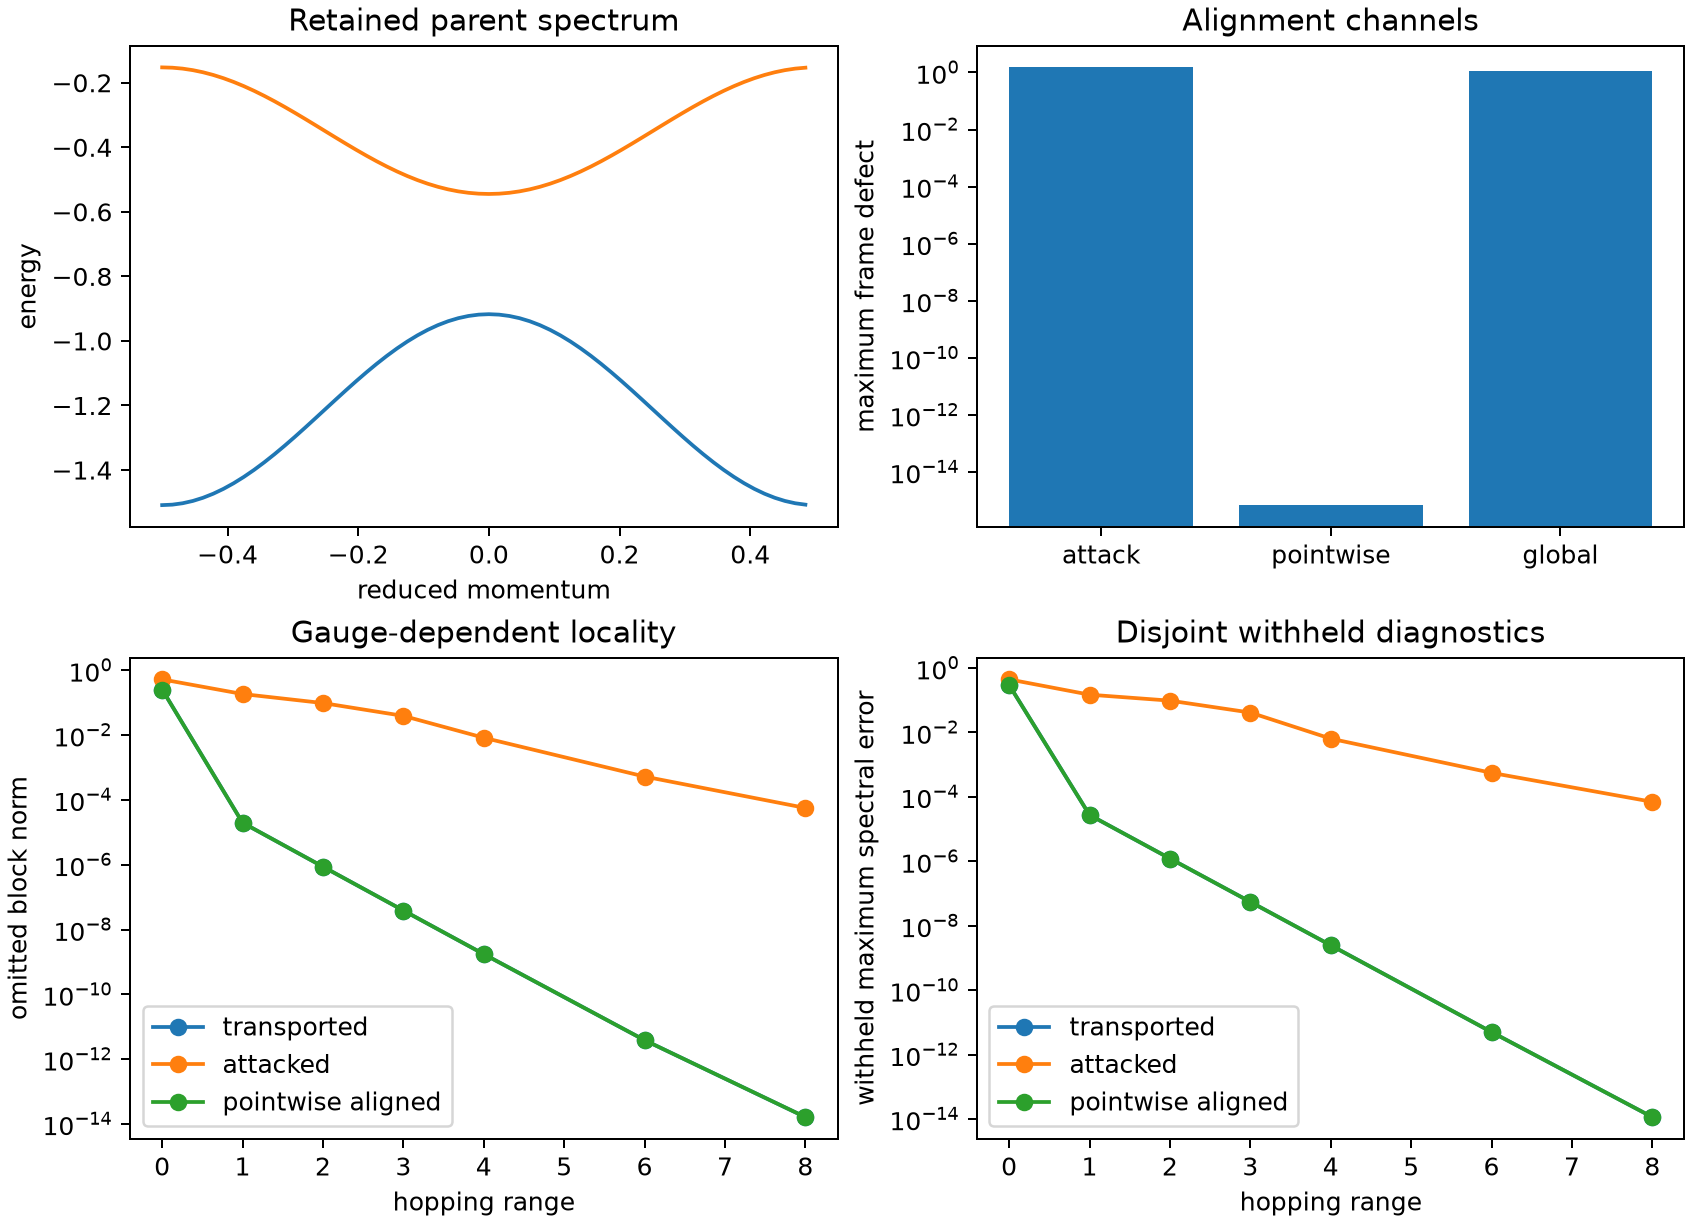
\includegraphics[width=0.97\linewidth]{../../../../../calculations/ICMSEP2026/conference/paper_1/multiband-alignment/multiband-alignment-summary.png}
 \caption{Frozen M2 retained spectrum, alignment channels, omitted block norms,
 and disjoint withheld maximum spectral errors. The exact pointwise channel is
 distinct from the one-global-unitary constrained family.}
 \label{fig:supp-m2-summary}
\end{figure}

\subsection{Gauge-resolved truncation and withheld checks}

Symmetric truncations retain representatives $|R|\leq R_{\max}$. Table
\ref{tab:supp-m2-ranges} reports selected values from the frozen range
sequence. The transported and pointwise-aligned frames recover the same local
behavior to floating-point error. In the attacked frame,
\[
 \widetilde H(k)=A(k)^\dagger H(k)A(k).
\]
Writing $H(k)=\sum_R e^{2\pi i kR}T_R$ and
$A(k)=\sum_m e^{2\pi i km}A_m$ gives the Fourier convolution
\[
 \widetilde T_Q=\sum_{m,n}A_m^\dagger T_{Q+m-n}A_n.
\]
A momentum-dependent unitary therefore mixes hopping coefficients across
ranges even though it preserves each fiber spectrum and retained projector; a
constant unitary has only its zero Fourier mode and merely conjugates each
block. Thus spectral and projector agreement do not protect finite-range
tight-binding locality or compressibility. The periodic attack redistributes
the same spectral information into a longer block-hopping tail. At range eight,
its omitted-block norm is $5.65\times10^{-5}$ and its withheld maximum spectral
error is $7.04\times10^{-5}$, compared with approximately
$1.6\times10^{-14}$ and $1.2\times10^{-14}$ for the transported channel.

\begin{table}[t]
\centering
\scriptsize
\caption{Selected M2 omitted-block norms and withheld maximum spectral errors.}
\label{tab:supp-m2-ranges}
\begin{tabular}{@{}rrrrrr@{}}
\toprule
$R_{\max}$ & $\|T\|_{\mathrm{omit}}$ & $\|\widetilde T\|_{\mathrm{omit}}$
& transported error & attacked error & aligned error\\
\midrule
0 & $2.54\!\times\!10^{-1}$ & $5.23\!\times\!10^{-1}$
  & $2.98\!\times\!10^{-1}$ & $4.45\!\times\!10^{-1}$ & $2.98\!\times\!10^{-1}$\\
1 & $1.98\!\times\!10^{-5}$ & $1.85\!\times\!10^{-1}$
  & $2.76\!\times\!10^{-5}$ & $1.49\!\times\!10^{-1}$ & $2.76\!\times\!10^{-5}$\\
4 & $1.75\!\times\!10^{-9}$ & $8.28\!\times\!10^{-3}$
  & $2.49\!\times\!10^{-9}$ & $6.43\!\times\!10^{-3}$ & $2.49\!\times\!10^{-9}$\\
8 & $1.63\!\times\!10^{-14}$ & $5.65\!\times\!10^{-5}$
  & $1.15\!\times\!10^{-14}$ & $7.04\!\times\!10^{-5}$ & $1.15\!\times\!10^{-14}$\\
\bottomrule
\end{tabular}
\end{table}

Withheld values evaluate only already fixed finite-range models. They do not
alter the parent, frame transport, attack, alignment family, hopping ranges,
thresholds, or figure-data selection.

\subsection{Independent verification and provenance}

The retained verifier independently rebuilds the parent polynomial,
eigenspaces, polar transport, periodic attack, pointwise and global
alignments, projected operators, Fourier blocks, Hermiticity defects,
truncations, omitted norms, and training/withheld spectral errors. Its maximum
dimensionless defect is $1.33\times10^{-15}$ and its maximum energy-channel
defect is $7.43\times10^{-15}$, both below the frozen $10^{-11}$ tolerance.

The input and protocol were hashed before the confirmatory calculation. The
package retains the protocol freeze, result, independent verification,
figure-data CSV, figure, report, software environment, source manifest, and
artifact checksums. The software record reports Python 3.14.6, NumPy 2.5.1,
SciPy 1.18.0, Matplotlib 3.11.1, and \texttt{ksdft2effmass 0.1.0.dev0}; the
dirty worktree is bound by \texttt{source.sha256}. No external calculator was
invoked.

\clearpage
\section*{Appendix S4. Wannier90 bridge calculation}
\label{supp:wannier90-bridge}
\renewcommand{\theequation}{S4.\arabic{equation}}
\setcounter{equation}{0}
\renewcommand{\thetable}{S4.\arabic{table}}
\setcounter{table}{0}
\renewcommand{\thefigure}{S4.\arabic{figure}}
\setcounter{figure}{0}

\subsection*{S4.1 Role and evidence boundary}

This appendix connects the controlled gauge-locality mechanism to retained
Wannier90 executions. It does not redefine M2. The balanced calculation is the
synthetic, non-DFT record
\path{research-monograph.periodic-2d.wannier90-balanced.v1} under
\path{calculations/research-monograph/periodic-2d/}. The parent is a finite
plane-wave representation of
\begin{equation}
 H=-\nabla^2+0.5\cos x+0.5\cos y+0.15\cos x\cos y
 \label{eq:supp-s4-parent}
\end{equation}
with a $15\times15\times1$ reciprocal mesh and a retained lowest-three-band
subspace. Wannier90 3.1.0 used centered $s$, $p_x$, and $p_y$ trial
projections; no disentanglement was used.

The external execution was historically authorized and retained. It is not
rerun by this manuscript. Repository-only verification consumes the compact
portable fixture and reconstructs the comparison independently of the
extractor. Passing establishes bounded consistency for this synthetic finite
interface, not first-principles, material, or general Wannier90 validation.

\subsection*{S4.2 Converged finite case and common-space alignment}

After a retained failed preprocessing attempt, the balanced auxiliary embedding
completed preprocessing and localization. Localization satisfied the frozen
$10^{-12}$ spread criterion at iteration 94. The direct projected frame and the
Wannier90 frame span the same retained subspace within a maximum projector
Frobenius defect of $2.65\times10^{-10}$.

Their raw represented Hamiltonians differ by $1.137E_G$ in maximum Frobenius
norm. Let $U_{\mathrm d}(\bm k)$ and $U_{\mathrm W}(\bm k)$ denote the direct
and Wannier90 frames. The pointwise unitary identification derived from those
frames reduces the represented-operator defect to
$3.57\times10^{-10}E_G$. By contrast, the frozen bounded family consisting of
independent integer orbital translations in $[-1,1]^2$ followed by one constant
orbital unitary leaves a per-orbital frame RMS defect of $1.188$ and an operator
defect of $1.490E_G$. Thus the observed relation is genuinely
$\bm k$-dependent within this comparison contract; it is not explained by a
single orbital rotation and bounded relabeling of orbital cells.

\subsection*{S4.3 Localization and hopping locality}

Native Wannier90 Berry-link spreads and common finite-supercell spreads use
different estimators and are not substituted for one another. The native total
active-plane spread is $0.7094a^2$. Under the common finite-supercell estimator,
the Wannier90 total is $6.1359a^2$ and the direct projected total is
$24.5163a^2$, giving a ratio of $0.2503$ for this finite case.

The same frame change also affects matrix-hopping tails. At squared-radius
shell 18, the omitted Frobenius $\ell^2$ norm is
$9.92\times10^{-3}E_G$ for the Wannier90 frame and
$1.38\times10^{-2}E_G$ for the direct projected frame. At shell 50 the values
are $2.72\times10^{-4}E_G$ and $5.90\times10^{-3}E_G$, respectively. These
commensurate diagnostics support the expected connection between localized
frames and shorter represented hopping tails for the frozen case. They do not
establish an optimality theorem.

The native \path{_hr.dat} blocks reconstruct the external mesh within
$3.06\times10^{-5}E_G$ in maximum Frobenius norm and
$2.23\times10^{-5}E_G$ spectrally. Those defects are retained as finite decimal
serialization effects, not relabeled as hopping truncation.

\begin{figure}[t]
 \centering
 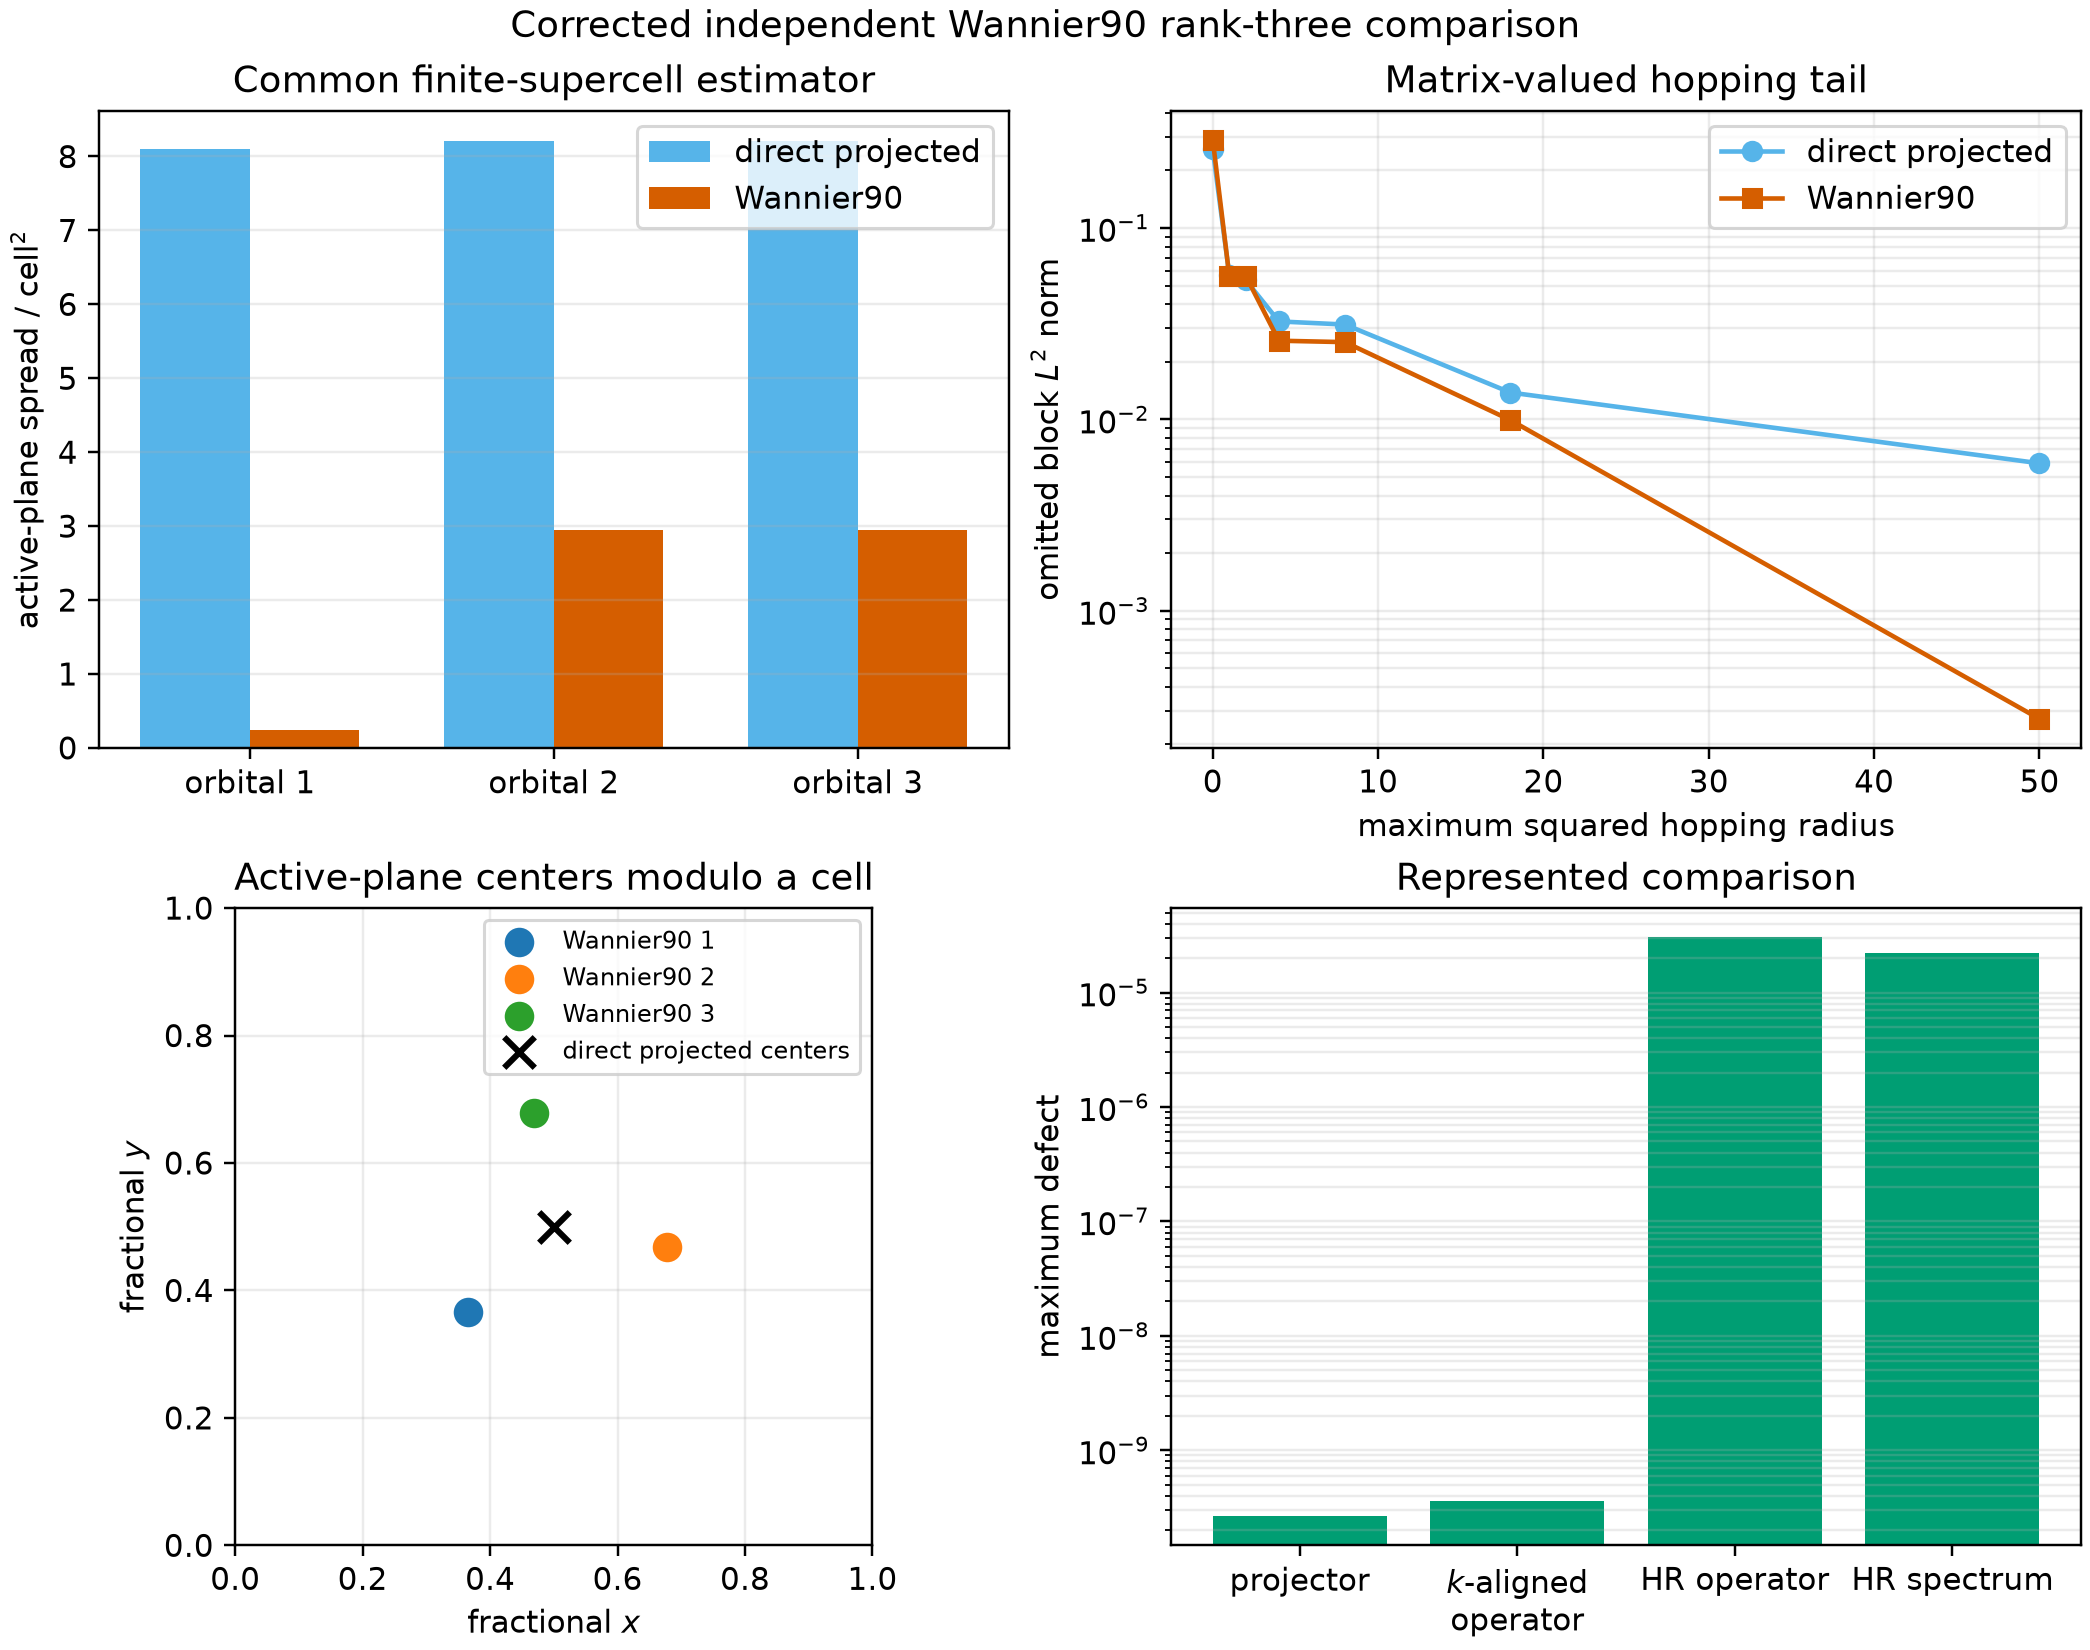
\includegraphics[width=0.97\linewidth]{../../../../../calculations/research-monograph/periodic-2d/wannier90-balanced-summary.png}
 \caption{Retained balanced Wannier90 comparison. Native and common-estimator
 spreads remain separate; aligned operator and shell-tail channels are evaluated
 on declared common representations.}
 \label{fig:supp-s4-wannier90-balanced}
\end{figure}

\subsection*{S4.4 Sensitivity study and interpretation limit}

A separately retained six-case study varies one of reciprocal mesh, plane-wave
cutoff, or inactive embedding length at a time. All finite cases converged, but
the outcomes are nonmonotone. Table~\ref{tab:supp-s4-sensitivity} records the
native spread and radius-50 tail needed for the interpretation boundary.

\begin{table}[t]
\centering
\small
\caption{Selected retained Wannier90 sensitivity observations.}
\label{tab:supp-s4-sensitivity}
\begin{tabular}{@{}lrr@{}}
\toprule
Case & Native spread ($a^2$) & Radius-50 tail ($E_G$)\\
\midrule
Reference $P3,N15,c15$ & $0.7094$ & $2.72\times10^{-4}$\\
Mesh $N=19$ & $1.7901$ & $4.52\times10^{-2}$\\
Cutoff $P=2$ & $1.7072$ & $3.30\times10^{-2}$\\
Cutoff $P=4$ & $1.7024$ & $3.38\times10^{-2}$\\
Embedding $c=12$ & $0.7093$ & $2.72\times10^{-4}$\\
Embedding $c=18$ & $1.7024$ & $3.38\times10^{-2}$\\
\bottomrule
\end{tabular}
\end{table}

The $c=12$ case returns close to the reference, whereas $c=18$ reaches a
different localization basin. The cutoff and mesh observations likewise do not
form a convergence sequence. Accordingly, the balanced calculation is a
positive finite-case bridge between M2's gauge mechanism and an actual
Wannier90-selected frame, while the sensitivity study blocks any claim of
mesh-, cutoff-, embedding-, or basin-independent localization. Neither record
supports a Si:P, Si:B, bulk-silicon, or other material-specific locality bound.

\subsection*{S4.5 Verification and provenance}

The portable balanced verifier independently reconstructs the finite parent,
direct polar frame, subspace and represented-operator defects, bounded
translation-plus-constant alignment search, native hopping reconstruction,
shell tails, convergence record, and common-grid densities and spreads. The
portable sensitivity verifier checks all six retained cases. Both pass against
the retained records. The directory-level \path{SHA256SUMS} manifest verifies
the reports, results, portable evidence, scripts, and figures. As in Appendix
S2, the digests establish byte consistency relative to the retained manifest;
they are not by themselves an external timestamp or a material-validation
argument.


\bibliographystyle{elsarticle-num}
\bibliography{references}

\end{document}
